% Template for Assignment Reports

\documentclass{article}

\usepackage{fancyhdr} % Required for custom headers
\usepackage{lastpage} % Required to determine the last page for the footer
\usepackage{extramarks} % Required for headers and footers
\usepackage{graphicx,color}
\usepackage{anysize}
\usepackage{amsmath}
% \usepackage{natbib}
\usepackage{caption}
\usepackage[hidelinks]{hyperref}
\usepackage{listings,fancyvrb}
\lstset{
  basicstyle=\ttfamily,
  columns=fullflexible,
  frame=single,
  breaklines=true,
  postbreak=\mbox{\textcolor{red}{$\hookrightarrow$}\space},
}
\usepackage{float}
\usepackage{lipsum}  
\usepackage{nameref}
\usepackage{pgf-umlsd}
\usepackage{subcaption}

% Margins
%\topmargin=-0.45in
%\evensidemargin=0in
%\oddsidemargin=0in
\textwidth=6.5in
%\textheight=9.0in
%\headsep=0.25in 
\renewcommand{\familydefault}{\sfdefault}
\usepackage[T1]{fontenc}

\linespread{1.0} % Line spacing

%%------------------------------------------------
%% Image and Listing code
%%------------------------------------------------
%%sw \includecode{caption for table of listings}{caption for reader}{filename}
\newcommand{\includecode}[3]{\lstinputlisting[float,floatplacement=H, caption={[#1]#2}, captionpos=b, frame=single]{#3}}


%%sw \includescalefigure{label}{short caption}{long caption}{scale}{filename}
\newcommand{\includescalefigure}[5]{
\begin{figure}[htb]
\centering
\includegraphics[width=#4\linewidth]{#5}
\captionsetup{width=.8\linewidth} 
\caption[#2]{#3}
\label{#1}
\end{figure}
}

%%sw \includefigure{label}{short caption}{long caption}{filename}
\newcommand{\includefigure}[4]{
\begin{figure}[htb]
\centering
\includegraphics{#4}
\captionsetup{width=.8\linewidth} 
\caption[#2]{#3}
\label{#1}
\end{figure}
}


%%------------------------------------------------
%% Parameters
%%------------------------------------------------
% Set up the header and footer
\pagestyle{fancy}
\lhead{\authorName} % Top left header
\chead{\moduleCode\ - \assignmentTitle} % Top center header
\rhead{\firstxmark} % Top right header
\lfoot{\lastxmark} % Bottom left footer
\cfoot{} % Bottom center footer
\rfoot{Page\ \thepage\ of\ \pageref{LastPage}} % Bottom right footer
\renewcommand\headrulewidth{0.4pt} % Size of the header rule
\renewcommand\footrulewidth{0.4pt} % Size of the footer rule
\setlength\parindent{0pt} % Removes all indentation from paragraphs

\newcommand{\assignmentTitle}{Assignment 2: Flow Forwarding} % Assignment title
\newcommand{\moduleCode}{CSU33031} 
\newcommand{\moduleName}{Computer\ Networks} 
\newcommand{\authorName}{Liam\ Junkermann} % Your name
\newcommand{\authorID}{19300141} % Your student ID
\newcommand{\reportDate}{\printDate}
\newcommand{\code}[1]{\texttt{#1}}

%%------------------------------------------------
%%	Title Page
%%------------------------------------------------
\title{
\vspace{-1in}
\begin{figure}[!ht]
\flushleft

\includegraphics[width=0.4\linewidth]{reduced-trinity.png}
\end{figure}
\vspace{-0.5cm}
\hrulefill \\
\vspace{0.5cm}
\textmd{\textbf{\moduleCode\ \moduleName}}\\
\textmd{\textbf{\assignmentTitle}}\\
\vspace{0.5cm}
\hrulefill \\
}

\author{\textbf{\authorName,\ \authorID}}

\date{\today}



%%------------------------------------------------
%% Document
%%------------------------------------------------
\begin{document}
\lstset{language=Java, captionpos=b, frame=single, keywordstyle=\color{black}\bfseries, stringstyle=\ttfamily}
\captionsetup{width=.8\linewidth} 

\maketitle
\tableofcontents
\vspace{0.5in}

\begin{abstract}
	This report will discuss the implementation of a flow forwarding software defined wide area system (SD-WAN). Starting with a brief overview of the theory needed to build and execute such a system, the components of the final implementation, a demonstration of a network topology employing this system, a brief discussion of potential improvements, and finally a summary and reflection of the assignment.
\end{abstract}

\newpage
%%------------------------------------------------
\section{Introduction}
%% The introduction should describe the general problem that should be addressed in the assignment, the approach that you have taken 
This assignment focused on the development and deployment of a flow forwarding mechanism to allow two clients (\code{End nodes}) on separate networks to interact as though they have a share network by employing a SD-WAN. A centralised \code{Controller} keeps track of the \code{Router}s and in turn the \code{End node}s attached to them. Messages are sent through an interactive console on the \code{End node} and then, with help from the \code{Router}s and \code{Controller}, directed to the appropriate \code{End node}.
This report will discuss the theory which led to the final implementation.

\vspace{1cm}
%%------------------------------------------------
\section{Theory}
%% The section on the theory at the basis of the assignment should describe the concepts and protocols that were used to realise a solution.
This flow forwarding implementation took inspiration from the OpenFlow \cite{openflow} protocol. Understanding this protocol has enabled me to lay the foundation for my implementation.

\subsection{OpenFlow}
\label{subsec:openflow}
This protocol was proposed as a way of allowing researchers to better test experimental protocols. Researchers found that the barrier to entry for new networking ideas was quite difficult as it is difficult to simulate the scale of a full-sized network. Therefore most new networking ideas go untested and therefore cannot make their way into production. OpenFlow addresses this by creating a standard for switches and communications which allow for programmable flow tables allowing the testing of new networking ideas. In practice OpenFlow leverages existing flow-tables built into ethernet switches and routers, this allows new protocols to be tested on a production network, while also allowing existing traffic to continue as normal. 

\vspace{1cm}
%%------------------------------------------------
\section{Implementation}
\subsection{Overview}
This implementation of the network uses some basic pieces from the proposed OpenFlow method. Specifically, \code{Router}s connect to the \code{Controller} with a \code{HELLO} packet, expecting a response in the form of a flow table (\code{FWD\_MOD}) update packet. This table is implemented statically for the purposes of this assignment. In the virtual network for this assignment I have implemented one \code{Controller} node and five \code{Router} nodes, these are started automatically by the \code{docker-compose.yml} file and run headlessly for the interactive \code{End Node} nodes to connect to. There are four \code{End Node} nodes also defined in the \code{docker-compose.yml} file, however these processes need to be started manually.

\subsection[Packet]{Packet Overview}
All packets have a two byte header, where byte index 0 is the packet type, and byte index one is the destination length. There are some cases where no destination is supplied, for example in the initial \code{Router} setup so this destination length packet allows data to be passed efficiently. This also allows for variable length destination names which is used in this implementation to mock different potential destinations in a humanly readable format. The packet types and their respective value are listed below:
\begin{lstlisting}[language=java,caption={[Encoded Packet Types]Code snippet from \code{Node} with the encoded packet types},label={lst:packet_types}]
  // Packet Types
  static final byte HELLO = 0;
  static final byte PACKET_IN = 1;
  static final byte FWD_MOD = 2;
  static final byte NETWORK_ID = 3;
\end{lstlisting}

All packets packets transmitted through this network follow the packet structure detailed in \autoref{fig:std_pkt}
\begin{figure}[!ht]
	\centering
	\begin{BVerbatim}
	 0                   1                   2                   3  
	 0 1 2 3 4 5 6 7 8 9 0 1 2 3 4 5 6 7 8 9 0 1 2 3 4 5 6 7 8 9 0 1
	+---------------------------------------------------------------+
	|                 |               |                             |
	|   PACKET TYPE   |  DEST LENGTH  |     DESTINATION/PAYLOAD     |
	|                 |               |                             |
	+---------------------------------+                             |
	|                                                               |
	|                      DESTINATION/PAYLOAD                      |
	|                                                               |
	+---------------------------------------------------------------+
	\end{BVerbatim}
	\caption{Standard Packet}
	\label{fig:std_pkt}
\end{figure}

\subsubsection[Operation]{Operation overview}
\autoref{fig:ex_seq} Shows the steps needed for the potential message to be sent from one end node to another.
The network deployed for this assignment is illustrated in \autoref{fig:network_diagram}. A controller is connected to each router as well.

\begin{figure}[!ht]
	\centering
	\begin{minipage}{.5\textwidth}
		\centering
		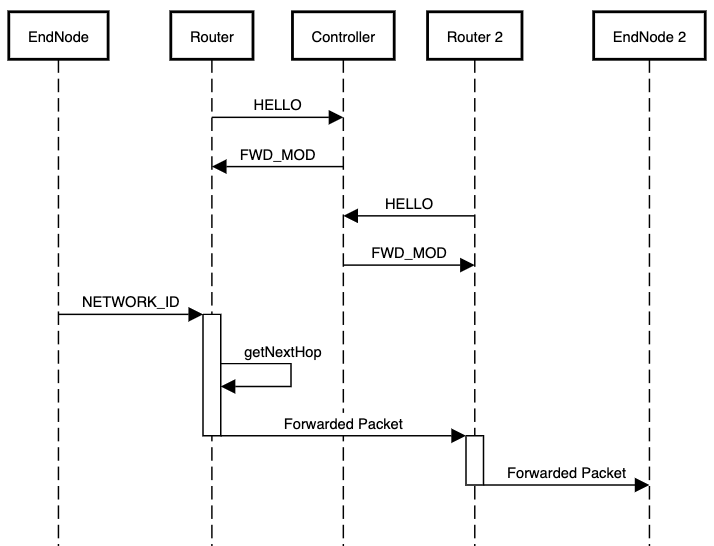
\includegraphics[width=0.8\linewidth]{ExampleSequence.png}
		\captionsetup{width=.6\linewidth}
		\captionof{figure}[Example Sequence Diagram]{A sequence diagram illustrating the setup and example message sharing between two end nodes}
		\label{fig:ex_seq}
	\end{minipage}%
	\begin{minipage}{.5\textwidth}
		\centering
		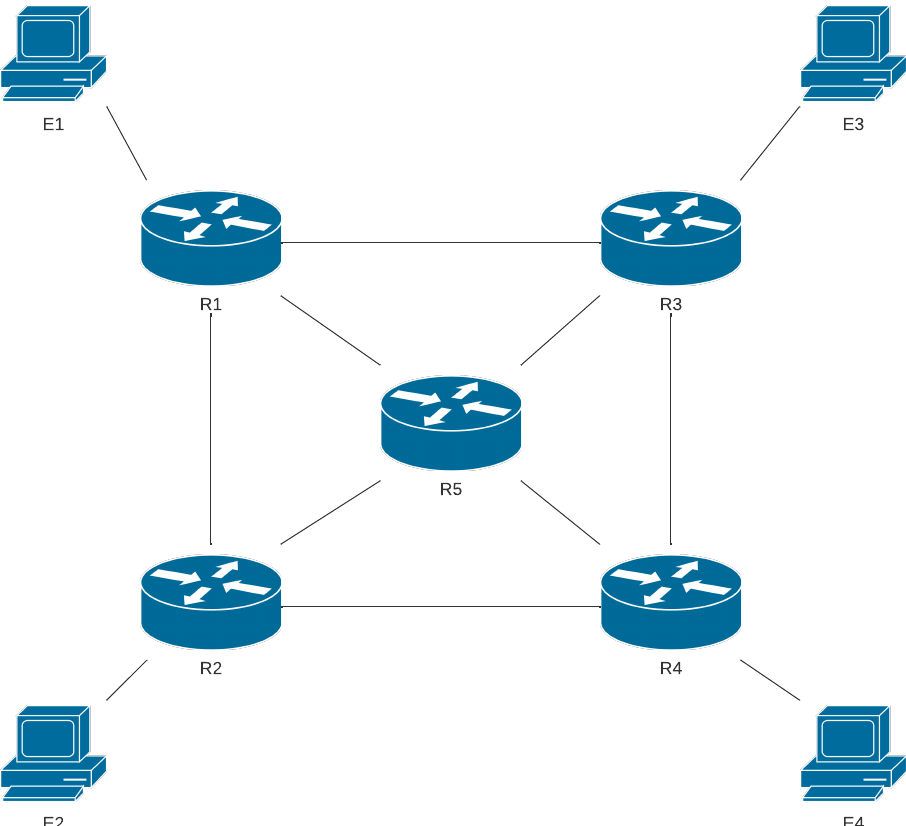
\includegraphics[width=0.8\linewidth]{NetworkDiagram.png}
		\captionsetup{width=.6\linewidth}
		\captionof{figure}[Network Setup]{An example network topology illustrating the interactions between nodes.}
		\label{fig:network_diagram}
	\end{minipage}
\end{figure}
This implementation only requires the destination to be included in the header as the flow table manages the output of each router based on the destination, source information would therefore be redundant for the purposes of forwarding messages. This decision will be discussed further in \nameref{sec:future_enhancements}. 
\begin{figure}[!ht]
	\centering
	\begin{minipage}{.5\textwidth}
		\centering
		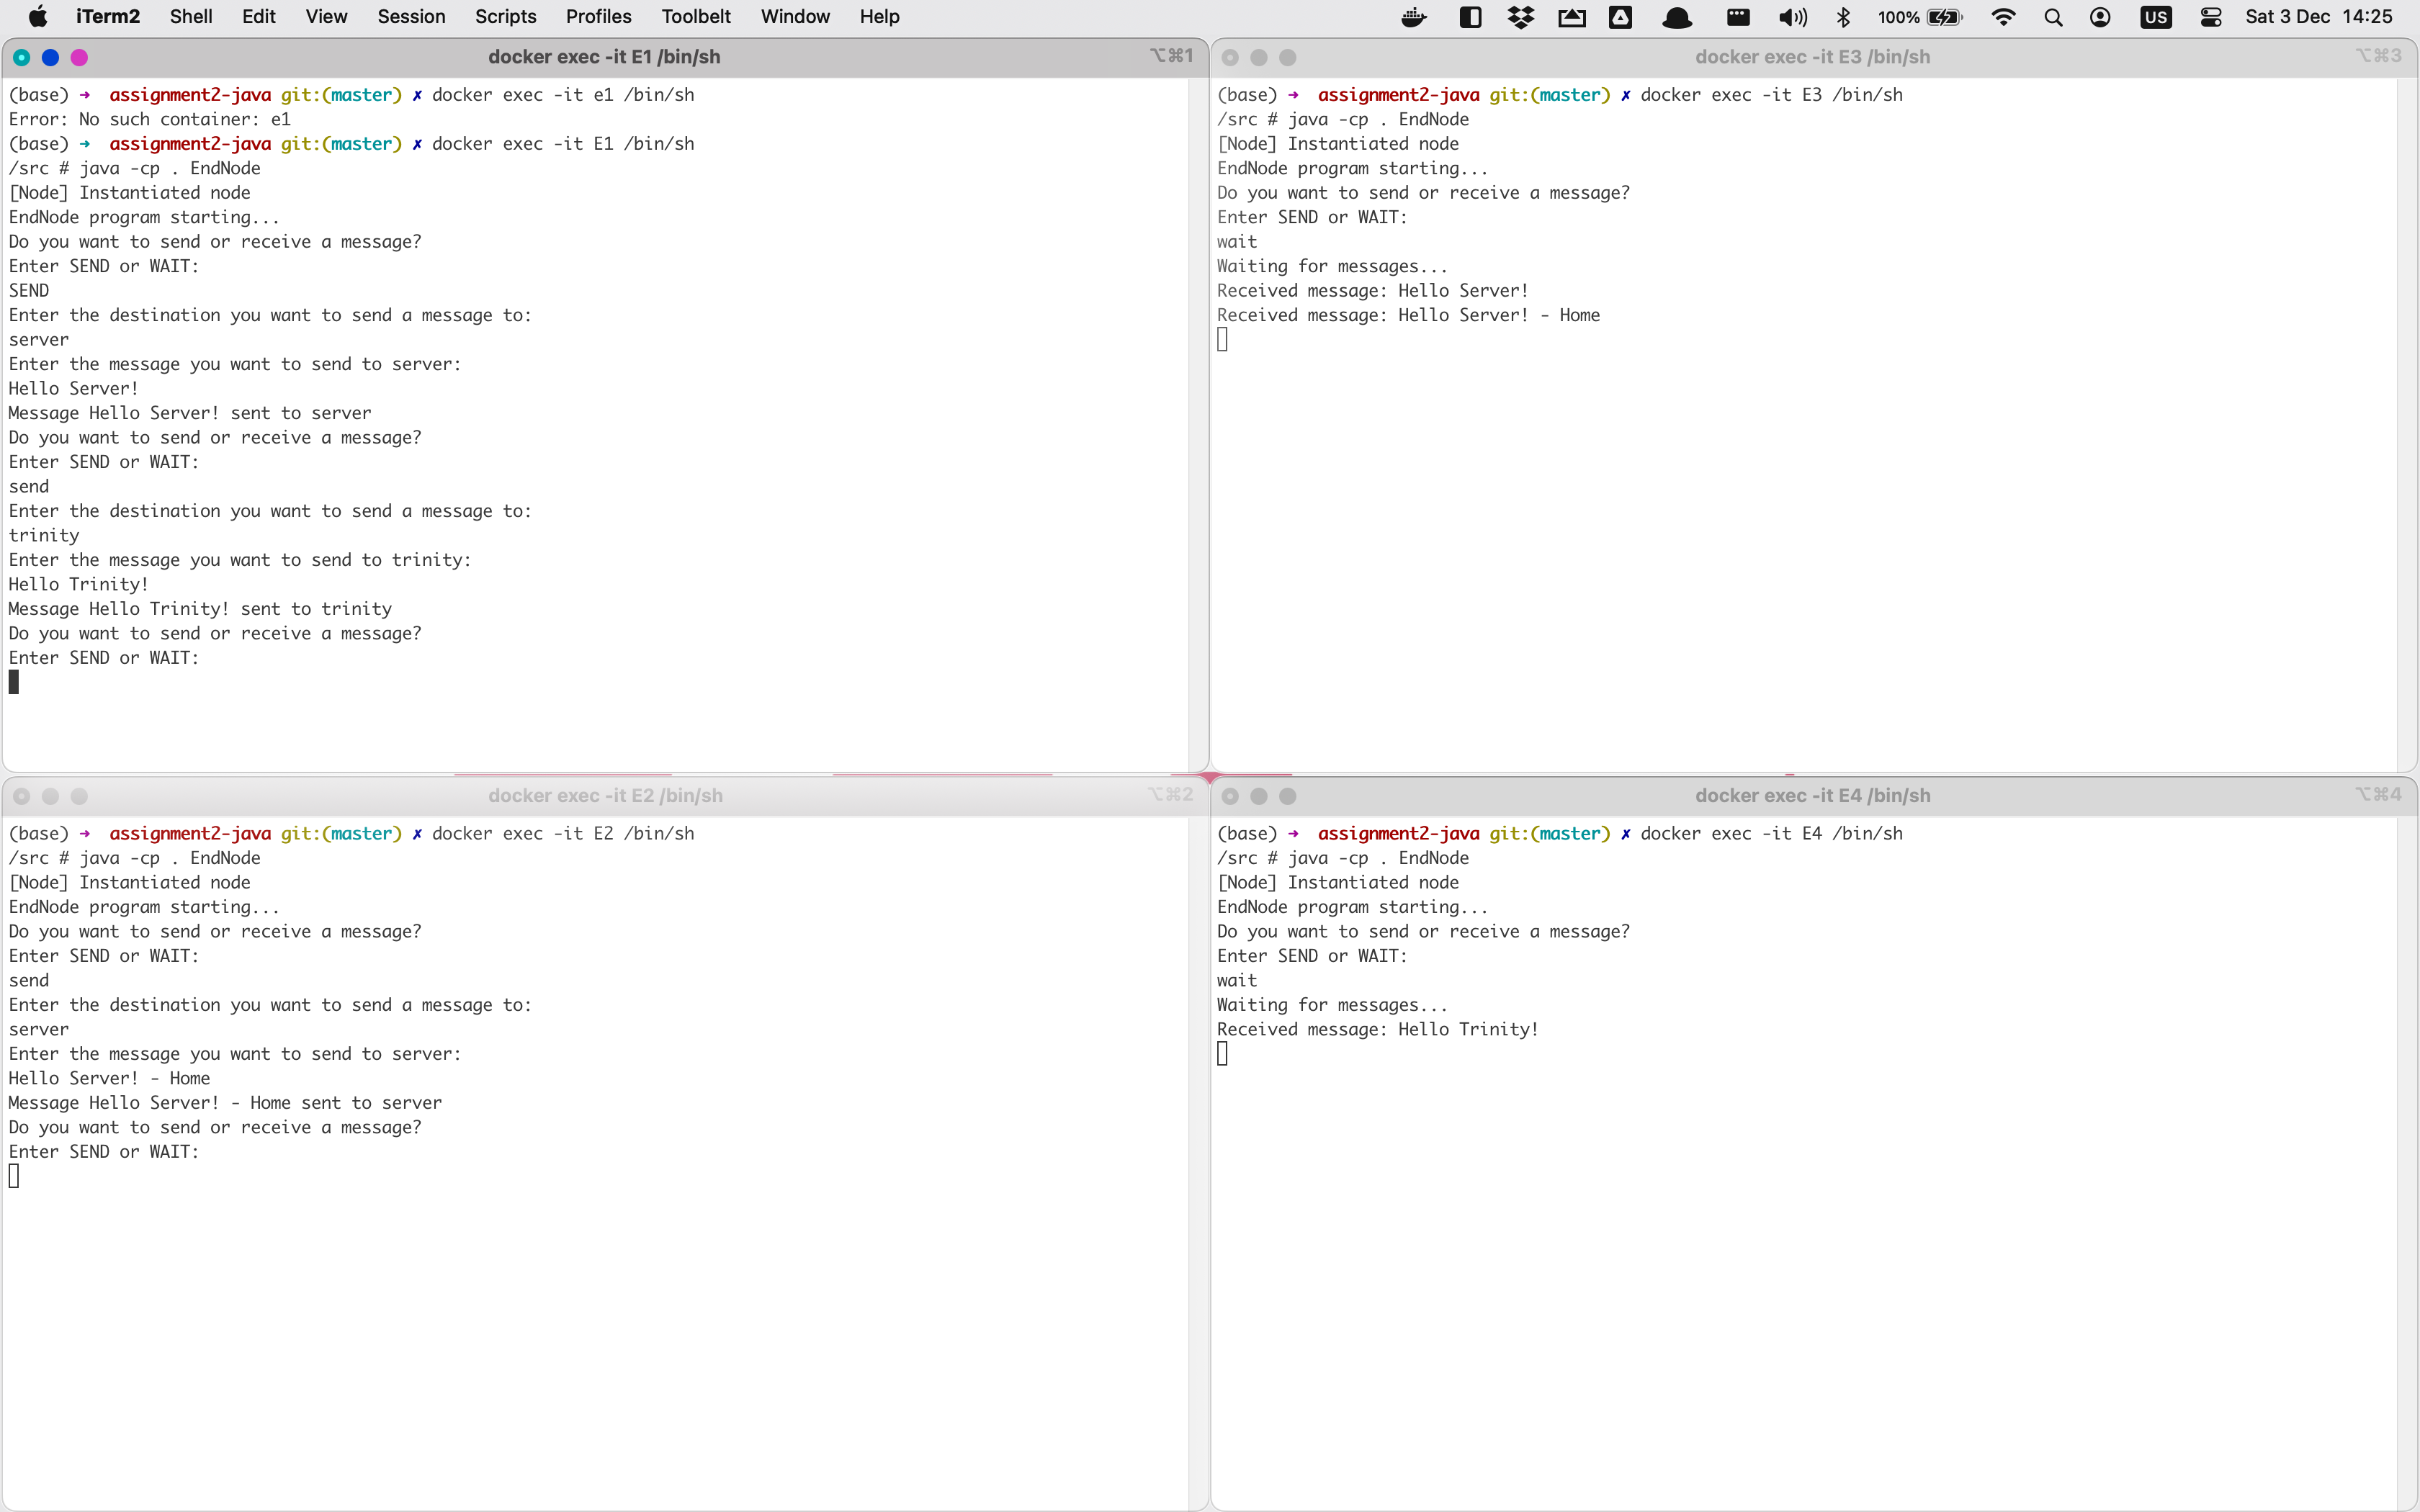
\includegraphics[width=0.8\linewidth]{term_usage.png}
		\captionsetup{width=.6\linewidth}
		\captionof{figure}[Example Usage]{Four terminals showing an example of the network usage with four mocked clients}
		\label{fig:term_usage}
	\end{minipage}%
	\begin{minipage}{.5\textwidth}
		\centering
		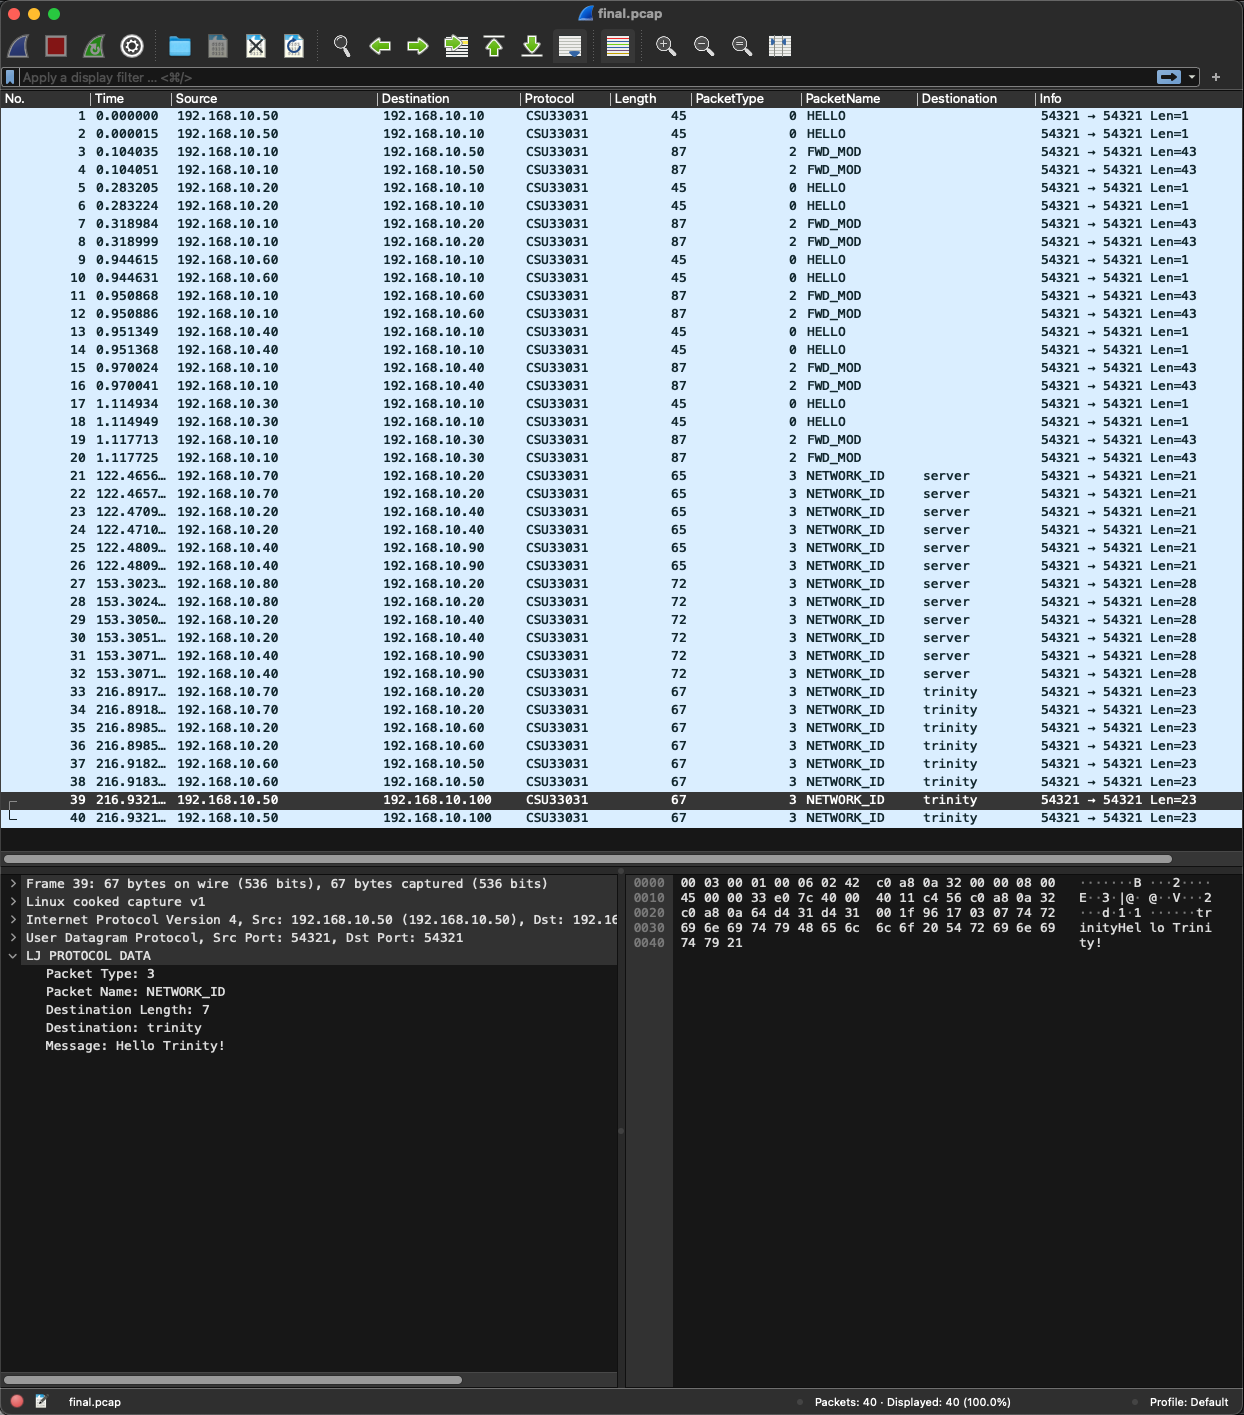
\includegraphics[width=0.8\linewidth]{pcap_output.png}
		\captionsetup{width=.6\linewidth}
		\captionof{figure}[PCAP File Output]{The packet capture of the example network usage}
		\label{fig:pcap_output}
	\end{minipage}
\end{figure}
\autoref{fig:term_usage} and \autoref{fig:pcap_output} show the client interface and packet capture of an example interaction in the virtual network.


\subsection{Network Components}
\subsubsection{Node}
\label{subsec:Node}
In practice each of these network nodes implement a \code{Node} class which handles most of the boilerplate Datagram behaviour and sets constants for header length, values, and positions, as well as providing some worker functions to generate packets and packet data appropriately. This \code{Node} also handles the multithreading needed to successfully multiplex within the \code{\nameref{subsec:Controller}}.

\subsubsection{Controller}
\label{subsec:Controller}
The \code{Controller} manages the forwarding table and helps routers resolve where packets should go when an entry may not be in the forwarding table. The \code{Controller} is initialised first in order to register \code{Router} nodes when receiving \code{HELLO} packets. The \code{Controller} also accepts \code{PACKET\_IN} packets which are also sent from the \code{Router}. This will be discussed further in the \nameref{subsec:Router} section. The forwarding table ahs been implemented statically as two dimensional array in the current implementation of the controller. This table outlines how each \code{Router} should direct a packet based on the destination value. The \code{Controller} is a headless node and is the first node started in the Docker Compose environment.

\subsubsection{Router}
\label{subsec:Router}
The \code{Router} node does most of the heavy lifting in this network, handling inputs from both \code{End Node} and other \code{Router} nodes and directing it appropriately. The \code{Router} handles two packet types:
\begin{description}
  \item[NETWORK ID] The \code{NETWORK\_ID} packet is sent from the \code{End Node} nodes with messages to forward to other nodes. The \code{Router} takes the data from the incoming packet and repackages it in a new packet with the next hop destination as described in the forwarding table which is received after the \code{Router} node starts up and makes contact with the \code{Controller}
  \item[FWD MOD] The \code{FWD\_MOD} packet is sent from the \code{Controller} and updates the forwarding table of the \code{Router} node. This \code{Router} can also receive this packet after forwarding a packet with an unresolved destination to the controller. This will be discussed further in \nameref{sec:future_enhancements}.
\end{description}

\subsubsection{End Node}
\label{subsec:EndNode}
The \code{End Node} handles the user input as well as displaying packets sent. As such, the \code{End Node} is fairly simple as it only expects to receive \code{PACKET\char`_IN} packets with messages. In this implementation, because all input is taken from a terminal based scanner, a client must opt to \code{WAIT} for messages, a feature which will be discussed further in \nameref{sec:future_enhancements}. Ordinarily, the user will enter whether they would like to send a message or wait for messages, if they choose to send messages they will be prompted to enter the destination, and the message. This interaction is exhibited in \autoref{fig:term_usage}.

\section{Future Enhancements}
\label{sec:future_enhancements}
This project is a simplified version of what a production ready release would look like. Therefore, some decisions were made to make the work more manageable. Firstly, the static forwarding table. Because I knew what the network topology would look like for this implementation I was able to create a static forwarding table. The first enhancement was I to continue this project would be to enable \code{Router} nodes to register with one another, and the \code{Controller} to allow new nodes to be added to the WAN. \code{End node} nodes would connect to the router and be added to the forwarding table dynamically allowing for a more flexible system. Next, the user experience would need to improve allowing clients to both view messages received and sent. This is more easily done when an application can handle both user input and network traffic separately as opposed to within the same terminal. Finally I would add a source header field to allow easier packet acknowledgement and response, but this would be built based on the needs of a given application.

%%------------------------------------------------
%% Summary of the document i.e. what was presented, what was the outcome of the project and the document.
\section{Summary}
In this report discussed the requirements for the assignment, the real-world version of a solution from which I drew inspiration, and finally my implementation of a flow forwarding mechanism. Then, an exploration of the basic functionality and an example topology of the completed network, as well as some limitations and potential improvements to this implementation.


%%------------------------------------------------
%% The reflection should layout your thoughts on the assignment
%% How many hours did you spent on the assignment? What worked well for you/what didn't?
%% What would you improve/change in your approach for the next assignment?
\section{Reflection}
Like the first assignment, this project had quite a large scope. Unfortunately during the period this assignment ran I fell somewhat behind in college work as a result of the sheer volume so I found if difficult to dedicate the time needed to execute this project with the same persistence and quality as the first assignment, this is reflected in the quality of this report. The expectations for each part of the assignment were clearer in this assignment though, which allowed me to be more organised in the final execution, and I should have used those opportunities more effectively. 


\bibliographystyle{plain}
\bibliography{refs}
\end{document}